\textbf{Qu'est-ce qu'un tromino ?}

Un \textbf{tromino} est une forme composée de trois carrés connectés par
leurs côtés. Dans ce problème, nous considérons uniquement les trominos en
forme de $L$, c'est-à-dire trois carrés formant un angle droit.

\textbf{Qu'est-ce qu'un pavage ?}

Un \textbf{pavage} consiste à recouvrir entièrement une surface avec des
formes sans chevauchement ni espace vide. Ici, nous cherchons à recouvrir une
grille carrée en utilisant uniquement des trominos.

\begin{center}
\resizebox{0.5\linewidth}{!}{%
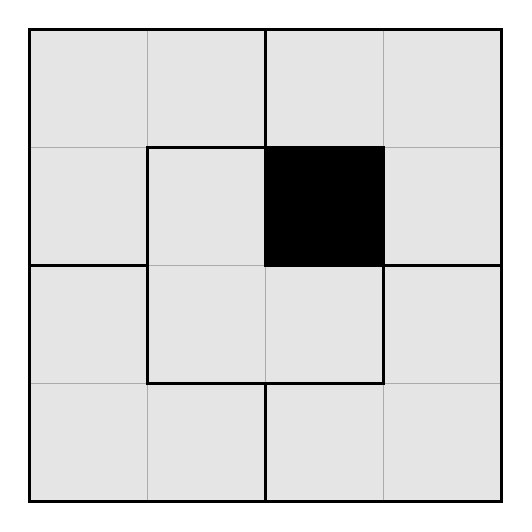
\begin{tikzpicture}[scale=1.5]
  \draw[very thick, fill=gray!20!white] (-2,0) -- (-1,0) -- (-1,1) -- (0,1) -- (0,2) -- (-2,2) -- cycle;
  \draw[very thick, fill=gray!20!white] (0,-2) -- (2,-2) -- (2,0) -- (1,0) -- (1,-1) -- (0,-1) -- cycle;
  \draw[very thick, fill=gray!20!white] (2,2) -- (2,0) -- (1,0) -- (1,1) -- (0,1) -- (0,2) -- cycle;
  \draw[very thick, fill=gray!20!white] (-2,-2) -- (-2,0) -- (-1,0) -- (-1,-1) -- (0,-1) -- (0,-2) -- cycle;
  \draw[very thick, fill=gray!20!white] (-1,-1) -- (1,-1) -- (1,0) -- (0,0) -- (0,1) -- (-1,1) -- cycle;
  \draw[opacity=.25] (-2,-2) grid (2,2);
  \draw[fill=black] (0,0) rectangle (1,1);
\end{tikzpicture}}
\end{center}

On considère une grille carrée de taille $2^n \times 2^n$, où $n$ est un
entier positif. Un des carrés de cette grille, quelconque, est colorié en noir. Chaque tromino
peut être tourné et doit couvrir exactement trois cases de la grille.

\textbf{Question :} Montrer que, quelle que soit la case noire, il est possible de recouvrir tous les autres carrés de la
grille avec des trominos en forme de $L$, sans chevauchement et sans laisser
de case vide.
